
%(BEGIN_QUESTION)
% Copyright 2007, Tony R. Kuphaldt, released under the Creative Commons Attribution License (v 1.0)
% This means you may do almost anything with this work of mine, so long as you give me proper credit

Shown here is the faceplate of a digital electronic single-loop process controller:

$$\includegraphics[width=15.5cm]{i02373x01.eps}$$

State your best guesses as to the functions of all buttons on this controller.  In particular, elaborate on the difference between {\it Auto} and {\it Manual} modes, and which parameters the ``arrow'' buttons affect.

Also, describe what steps an operator would have to take to switch this controller from automatic to manual modes, and manually change the output signal going to the control valve, and describe a practical situation where the operator might be inclined to do such a thing.

\underbar{file i02373}
%(END_QUESTION)





%(BEGIN_ANSWER)

\begin{itemize}
\item{} ``Displ'' button = {\it change display mode}
\item{} ``Auto/Man'' button = {\it toggle between automatic and manual modes}
\item{} ``Config'' button = {\it Enter the configuration menu}
\end{itemize}

\begin{itemize}
\item{} ``Up'' ($\uparrow$) Button = {\it increase setpoint}
\item{} ``Down'' ($\downarrow$) Button = {\it decrease setpoint}
\item{} ``Left'' ($\leftarrow$) Button = {\it decrease output}
\item{} ``Right'' () Button = {\it increase output}
\end{itemize}

\vskip 10pt

An operator might wish to manually control a process in the event that the transmitter providing the process variable (PV) signal fails.

%(END_ANSWER)





%(BEGIN_NOTES)

%INDEX% Basics, control: controller faceplate

%(END_NOTES)


